%-------------- Hardware Description ------------------ %
\section{Implementation}
Overview of the test setup can be seen in Fig- \ref{fig:fss_setup}, implementation can be divided in three parts
\begin{enumerate}
\item \textbf{Full Spectrum Simulator (FSS):} Which will have the power system model, through which different test conditions will be given
\item \textbf{PMU:} Which will consist of a ADC interfacing board and OMAP-L 137 EVM
\item \textbf{PC:} It will have a Phasor Data Concentrator (PDC), which receives data from the PMU and record it for future analysis.
\end{enumerate}
During the initial phase of the project, intention was to use indigenously PMU developed C-DAC but due to the hardware issues and lack of documentation and support, it was decided that a minimalistic PMU will be developed by ourself. Now we will see detailed description of each devices: 

\begin{figure*}[th]
\centering
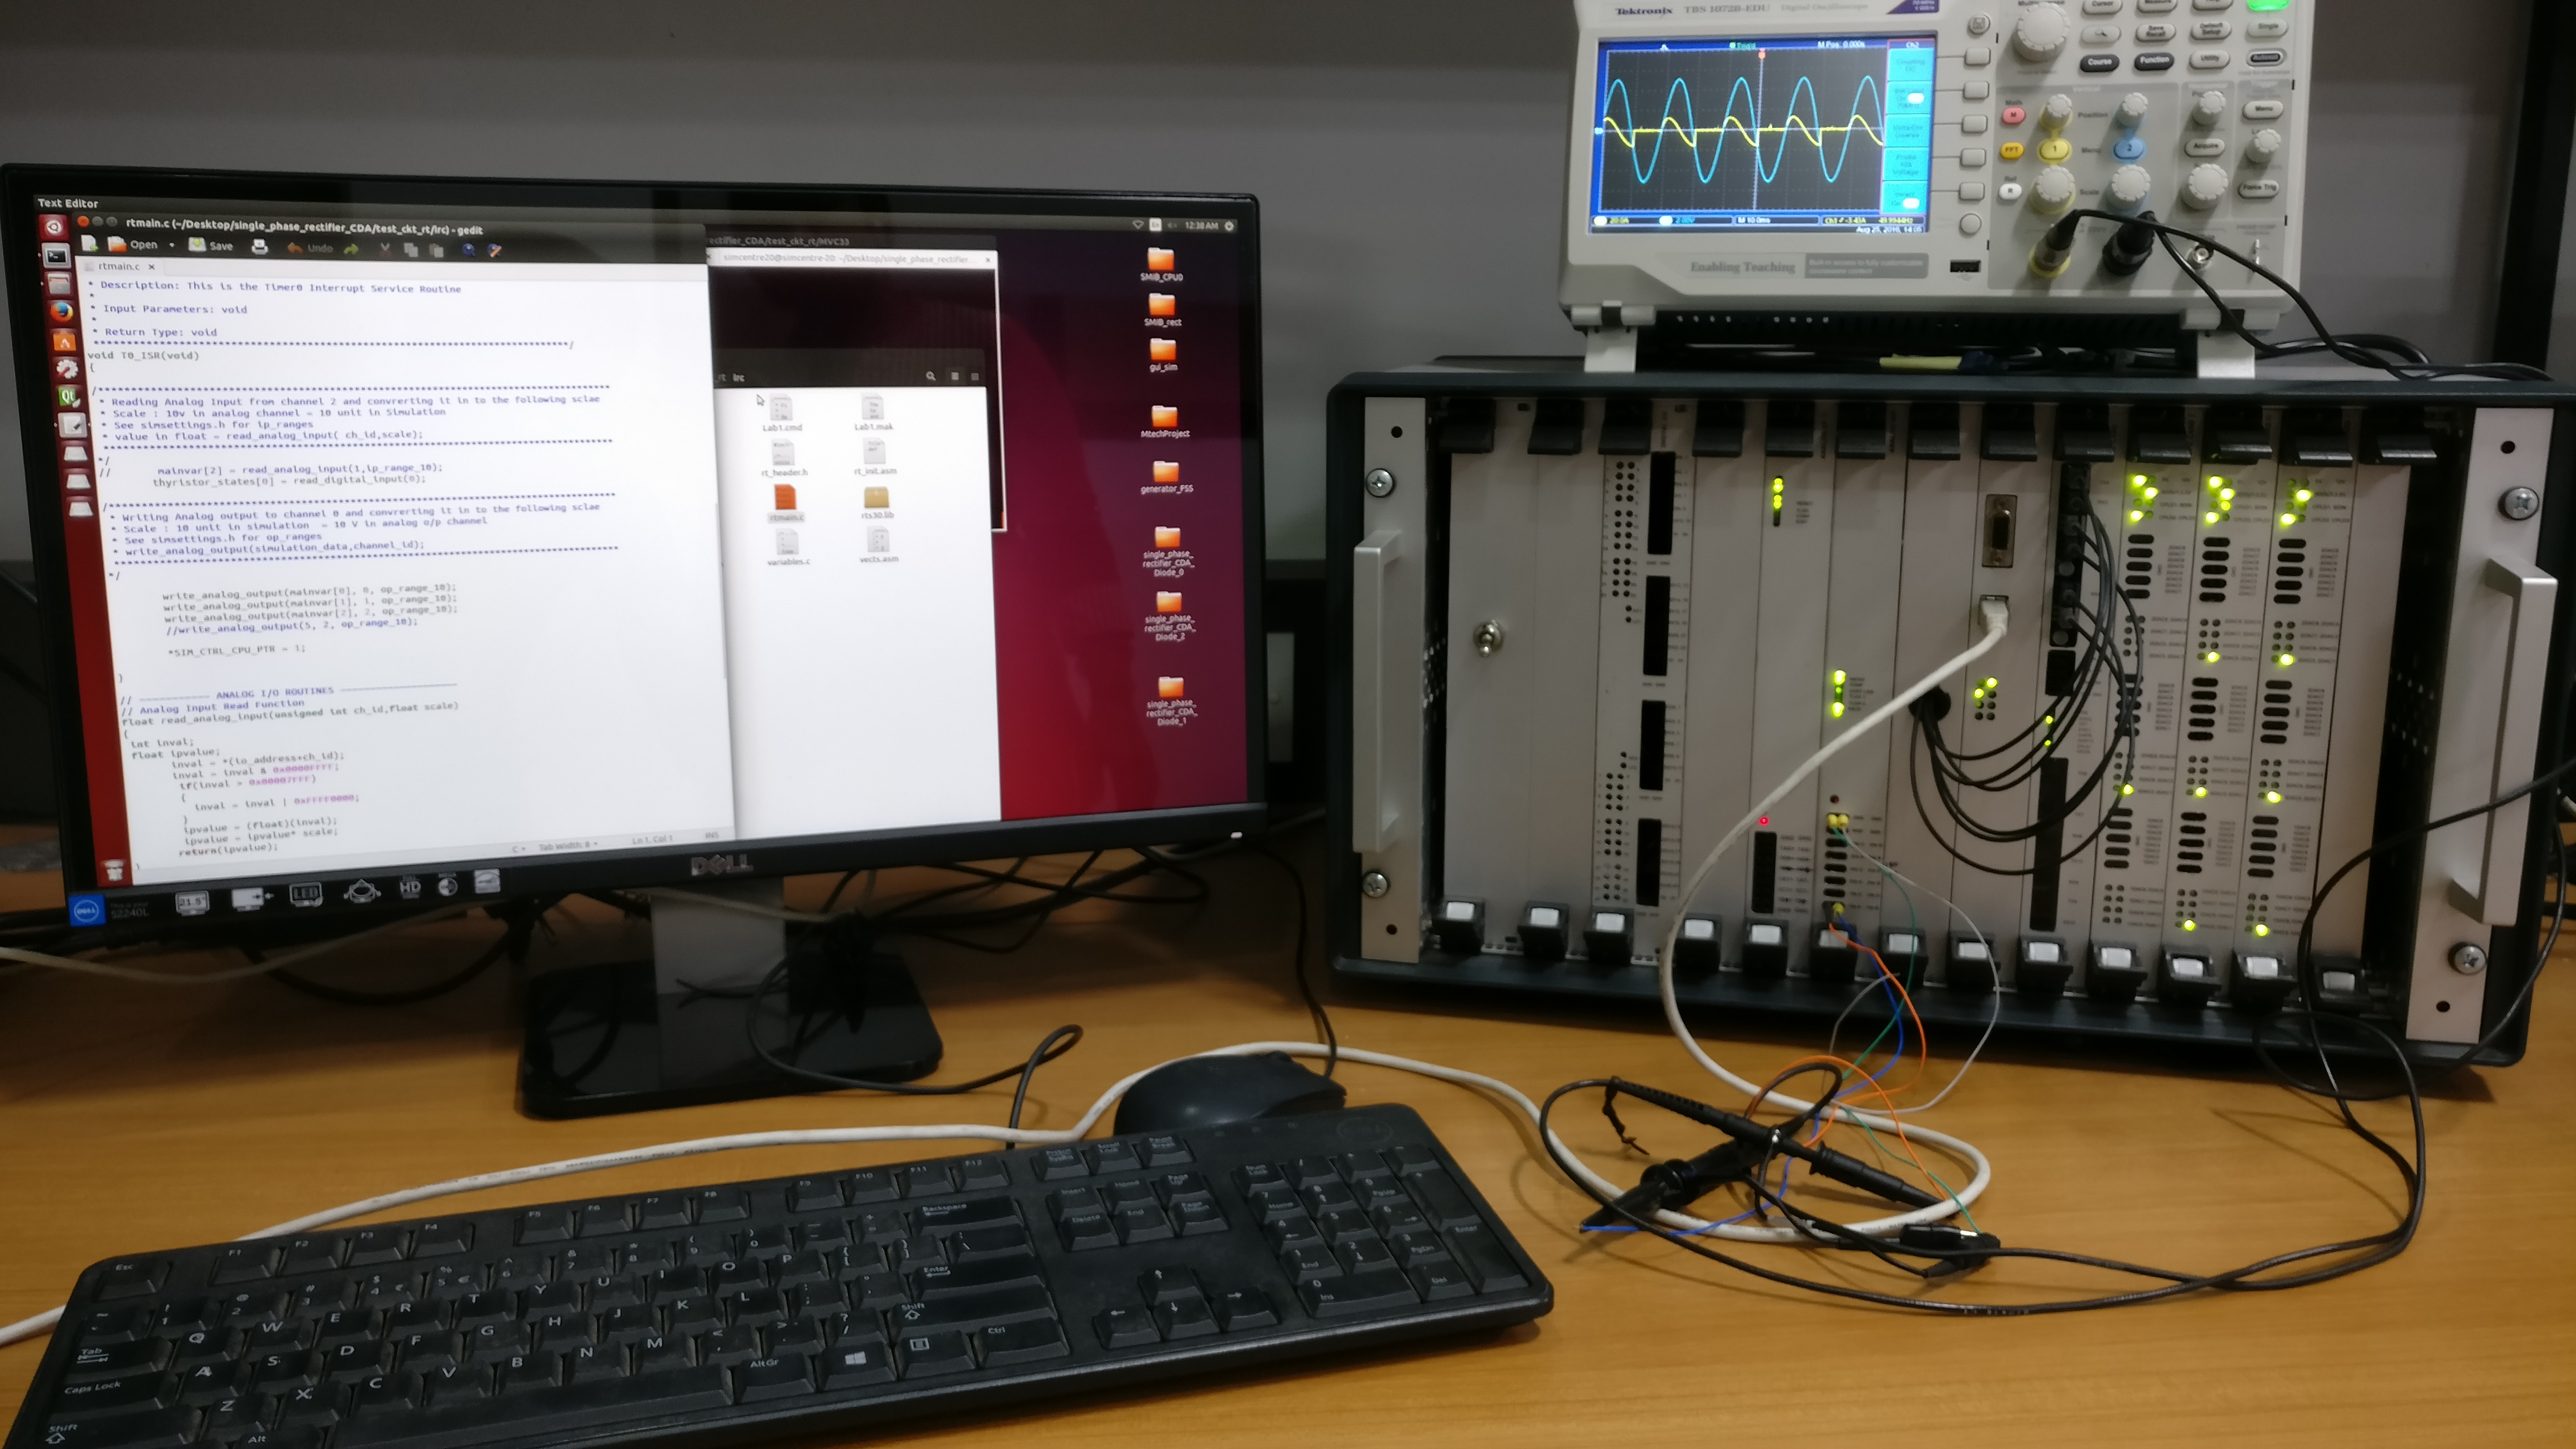
\includegraphics[width=\textwidth]{fig/FSS_setup.jpg}
\caption{Mini-FSS setup in laboratory}
\label{fig:fss_setup}
\end{figure*}

\subsection{Full Spectrum Simulator:}
As per the requirement of the implementation, miniature-Full spectrum Simulator will be used for this purpose. FSS is a card based, multi CPU - parallel processing hardware. It uses TI's MSP430 DSPs as building block. It was developed by IIT Bombay and CDAC for both, offline \& real-time  simulation purposes in Power Electronics and Power Systems.

\begin{figure}[th]
\centering
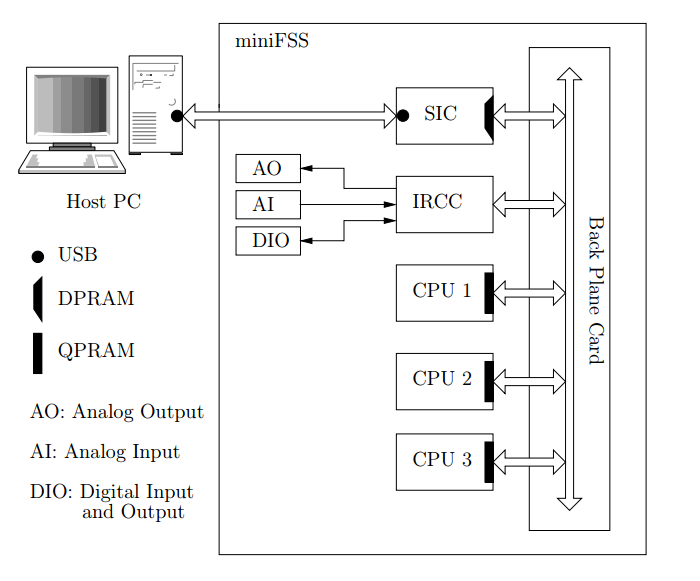
\includegraphics[width=250pt]{fig/fss_arch2.png}
\caption{FSS architecture}
\label{fig:fss_arch}
\end{figure}
As shown in Fig: \ref{fig:fss_arch} above it is a card base setup which contains:



\begin{itemize}
\item[-] System Interface Card (SIC)
\item[-] Intra Rack Control Card (IRC Card)
\item[-] Three CPU Cards (CPU 0, CPU 1 and CPU 2), each having 3 digital signal processors on it. So there are total 9 processors allowing for parallel computation.
\item[-] One Analog Output Card (AO Card), having 6 analog output channels (±10 V range).
\item[-]One Analog Input Card (AI Card), having 6 differential analog input channels (±10 V range).
\item[-] One Digital Input/Output Card (DIO Card), having 24 digital inputs and 24 digital outputs (0 - 5 V).
\item[-] One Back Plane PCB.
\end{itemize}

\begin{itemize}
\begin{figure}
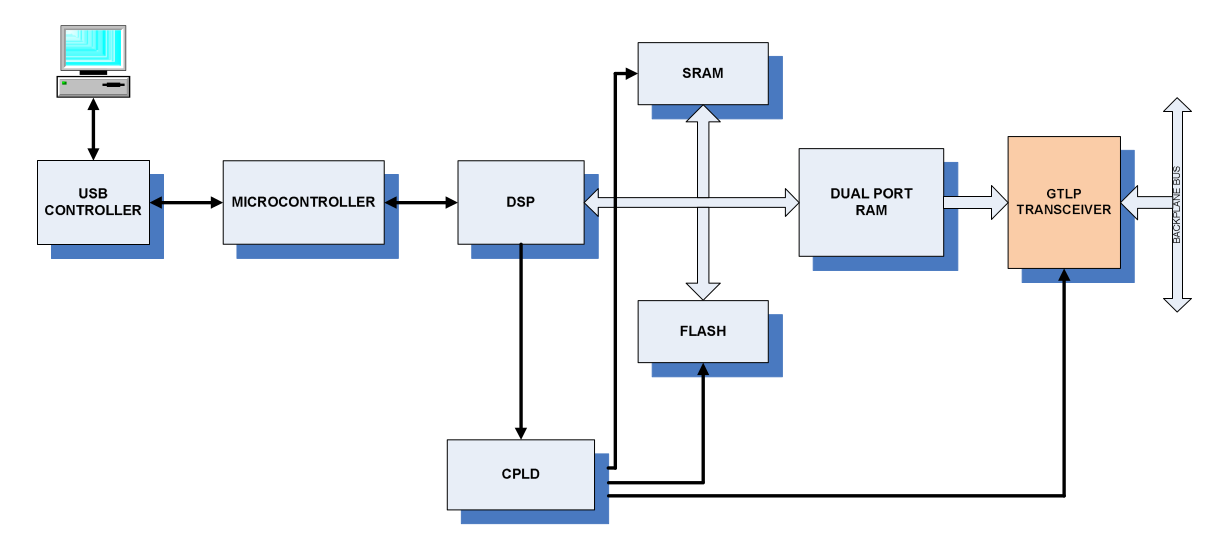
\includegraphics[width=\columnwidth]{fig/SIC_arch.png}
\caption{SIC block Diagram}
\label{fig:SIC}
\end{figure}

\item \textbf{System Interface Card:} 
It is called SIC, it acts as a communication layer between host PC and the CPUs in the CPU rack. It consists of TUSB chip which connects the device to host PC, real-time simulation software is downloaded to from the host computer to SIC over this USB interface for distribution over different CPUs. It communicates to other CPUs in the rack over backplane through Gun Transistor Logic Plus (GTLP) transceivers. A TMS320 chip is also there to interface SIC with IRC card and a MSP430 to have RS-232 interfacing.
\begin{figure}[ht]
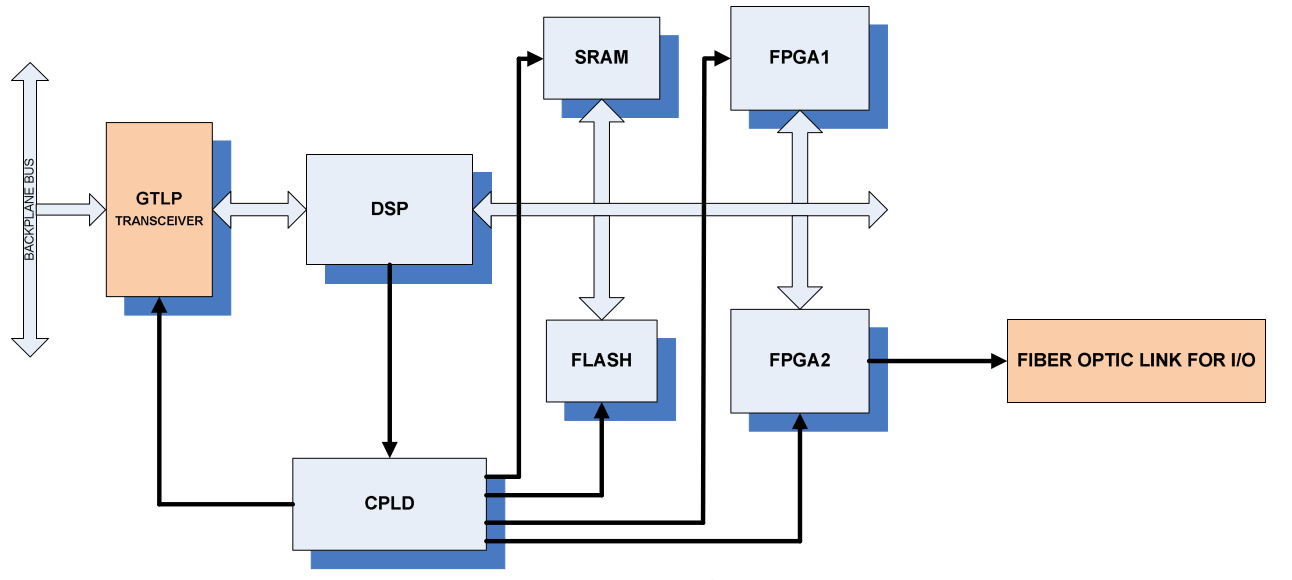
\includegraphics[width=\columnwidth]{fig/iirc_arch.png}
\caption{IIRC card Block Diagram}
\label{fig:IIRC}
\end{figure}

\item \textbf{Inter Intra Rack Communication Card:} IIRC is designed as a master controller card, which controls other cards, peripheral communication, timer triggered execution and host pc communication. Further more IIRC card handles analog as well as digital input-output also. Apart from that IIRC processor also controls the simulation execution using it's timer on the respective CPU card. IIRC card has protocol implemented to communicate between CPU cards and SIC so that simulation can be controlled and it's result can be sent to respective peripheral and/or can be downloaded to host PC.The communication to and from the I/O system over a high speed fiber optic network is also controlled by the IIRC cards using 2 Altera make FPGAs.

\begin{figure}[ht]
\includegraphics*[width=\columnwidth]{fig/cpu_card_arch.png}
\caption{CPU card Block Diagram}
\label{fig:cpu}
\end{figure}

\item \textbf{CPU card:} 
mini-FSS has 3 CPU cards, each having TI's MSP430 DSPs. These cards are heart of FSS. They handle all the mathematical algorithm associated with the simulation. Data flowing from and to the cards are controlled by IRC card via \textbf{back plane} PCB.
\end{itemize}

FSS having card base architecture with multiple CPU makes it a very viable platform for modeling purposes, as the system can be split across multiple process threads and concurrent execution can be done. This feature makes it extremely suitable for Power system and power electronics application as there different system cutset can be made to execute on each processor and hence results can be computed/ solved very fast. This feature is explored for the PMU testing as the system model is implemented over several cores/processors.

For our purposes in the beginning FSS will be used a real-time player only. A simulation will be developed in a Elector Magnetic Transient Program (EMTP) for a sample system, and it's data will be taken. This data will be used to create a output pattern to be played in real-time to the PMU. Latern on as the concept evolves A model of a small system (say 4 bus or more) will be implemented which will use multiple CPU cards and processors, which will used as an input to the PMU. Different kinds of transient conditions can be created using this, which can be later used for testing of the PMU.

Though as of now it has been observed that simulation having anything more than 2 bus is not possible to run due to step size and other technical aspects. But later on a more thorough effort will be made to implement it.

\subsection{PMU}
OMAP-L137 EVM is being used as the platform to design PMU. OMAP-L137 EVM doesnt have Analog to Digital Converter on board hence an interfacing circuit is developed. While designing the ADC board following criteria were kept considered.
\begin{itemize}
\item Good sampling rate: ~200 Samples/Sec
\item No of channels: 3 + 3 = 6 (3 - $\phi$ voltage and current) 
\item Interfacing type: It should be memory addressable and voltage level compatible  to the EVM.
\item Input type: FSS analog output is differential which can be configured as single ended, its voltage level is $\pm$10V
\end{itemize}

\begin{figure}[ht]
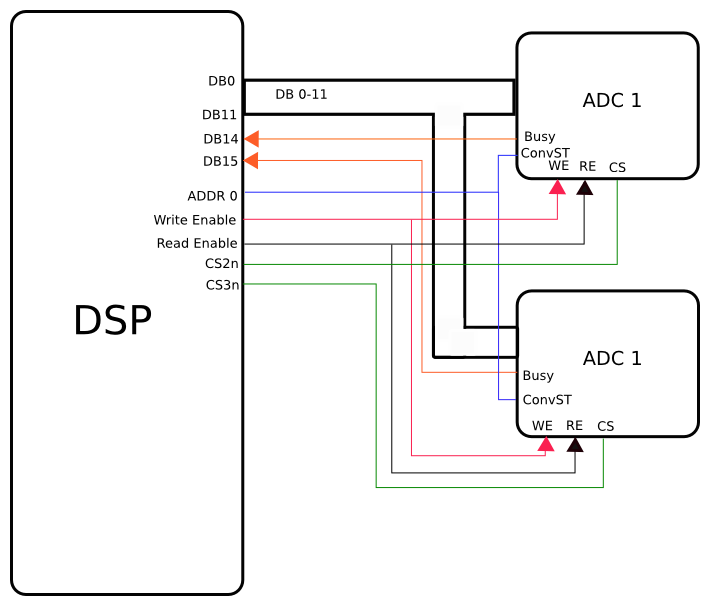
\includegraphics[width=\columnwidth]{fig/ADC_board.png}
\caption{ADC Board block diagram}
\label{fig:adc_board}
\end{figure}
Above Fig: \ref{fig:adc_board} shows the design logic of ADC board. Two AD7864-1 are used as ADC chips due to their high sampling rate of 500 ksps and direct input voltage compatibility range of $\pm$ 10 V. AD7864 is a high speed 4 channel simultaneous sampalling successive approximation ADC with \textit{bi-polar input} having conversion time as low as $1.65 \mu sec$. Chip's conversion sequence can be controlled through hardware as well as software, its default operating voltage is 5v but has a special output voltage shifter for interfacing it with 3.3v processors and controllers. This ADCs are fairly advance hence they have been interfaced with a special asynchronous peripheral interfacing architecture called EMIF-A, which is exclusively available in OMAP-L13x series processors. Extended Memory InterFace (EMIF) has two parts A \& B out of which EMIF-B is having \textit{Enhanced Direct Memory Access} controller (EDMA3) which enables the processor for multi-threaded rapid memory access and hence it is exclusively for highspeed SDRAM interfacing where as interface \textit{A} (EMIF-A) is developed for generic purposes more details are given below:

\subsubsection{EMIF-A}
EMIF-A controller is a 16-bit databus based versatile controller \cite{uguide:emifa}, designed to interact with variety of devices like 
\begin{itemize}
\item Single Data Rate (SDR) RAM
\item Asynchronous devices like NAND \& NOR flash memory and SRAM
\end{itemize}
It contains lot of features to ease and facilitate the usage of asynchronous devices. A functional block diagram is given here in Fig: \ref{fig:EMIFA} 
It is apperent from figure-\ref{fig:EMIFA}, that it has 4 cheap selects and, one read and write and 16 data channels. which makes it very convenient for interfacing multiple peripherals at a time. 
\begin{figure}[ht]
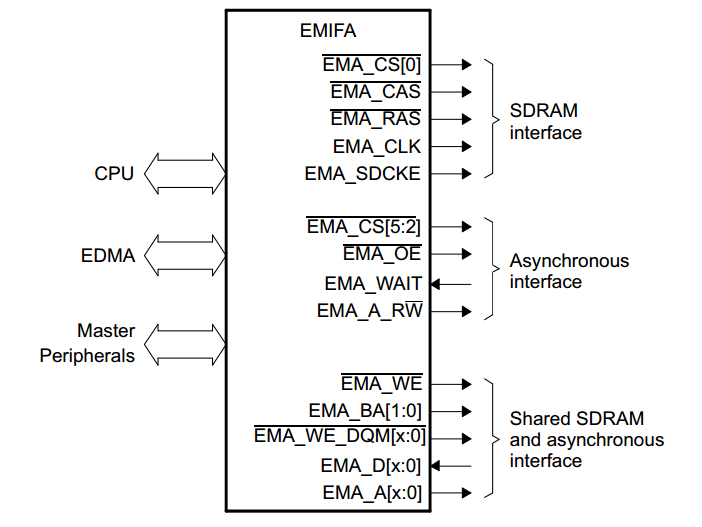
\includegraphics[width=\columnwidth]{fig/EMIFA.png}
\caption{EMIFA Block Diagram \cite{uguide:emifa} }
\label{fig:EMIFA}
\end{figure}

\subsubsection{ADC board Logic}
Due to EMIFA, interfacing of ADC board became quiet convenient rather than using pins in GPIO mode. So the logical flow of the board is as follows:

\begin{itemize}
\item 6 input channels are required hence 2 ICs are used
\item Chip Select (CS), Read, Write, and databits from 0 - 11 are directly available from the EMIFA interface, and they are shared with both the chips.
\item AD7864 has sequence selection which has been configured through hardware, and Clock source has been kept internal. because of this both the pins \texttt{INT/EXT\_CLK} \& \texttt{H/S select}
\item AD7864 has 3 control output \texttt{Busy}, \texttt{FIRSTDATA} and \texttt{EOC}. Out of these only \texttt{busy} is observed via a data line (data bits 16 \& 15). Data is \textbf{and}ed is not read until data line 15 \& 14 are not zero.
\item AD7864 supports two kinds of data reading 1) Reading during the conversion 2)Reading after the conversion. Here we are going to use \textit{Reading After the conversion}, below is the timing diagram of the chip for understanding the proper functioning of the circuit.
\end{itemize}
\begin{figure}[h]
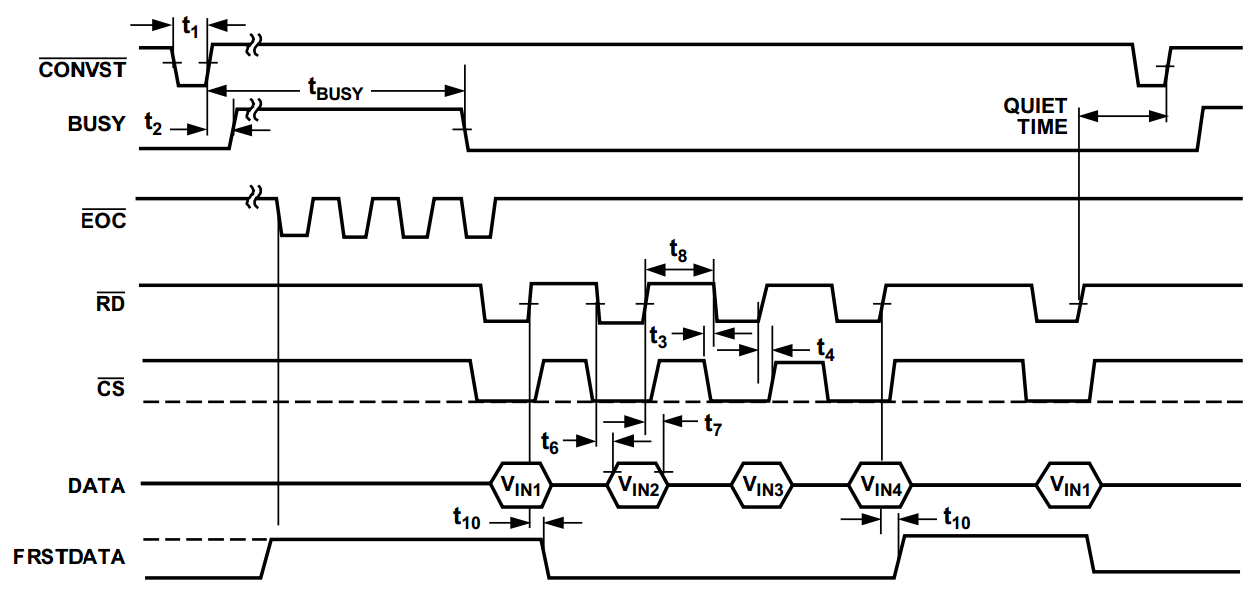
\includegraphics[width = \columnwidth]{fig/adc_time_diag.png}
\caption{ADC Reading After the Conversion timing }
\label{fig:adc_timing}
\end{figure}
Now we will see the operation that takes place when sampling  is to be done:
\begin{itemize}
\item Assert start of conversion (\texttt{CONVST}) is asserted via \texttt{EMA\_CS(4)}
\item Due to this chip will start the conversion processes which will make \texttt{BUSY} high,
\item Status of \texttt{BUSY}  will be checked via \texttt{DB15} \& \texttt{DB14} pins of the EMIFA header, for both the chips untill they are \texttt{low} again.
\item The moment \texttt{BUSY} goes low, \texttt{EMA\_CS[2]} and \texttt{EMA\_A\_RE} are asserted with which AD7864 starts putting data on data lines. this processes of asserting is repeated for 4 times, for each channel. The same is done using \texttt{EMA\_CS[3]} for getting data from 2nd ADC chip.
\end{itemize}

Apart from ADC board another important component in PMU is GPS signal. A NavSynch CW-12TIM GPS receiver is will be interfaced. The receiver provides three type of output signal.
\begin{itemize}
\item 1PPS - Synchronized with the start of the UTC second
\item 10MHz FOUT - The maximum time interval error (MTIE) of this signal is 4us at the interval of 446.8 Ks.
\item UART - Data communication port for UTC data and other control/status information
\end{itemize}
The receiver has an on board RTC which maintains the time information in loss of satellite fix. Now we will see description of computer interface.

\subsubsection{Computer}
It will have the Phasor Data Concentrator (PDC) program, which will collate the data coming from our PMU coming over serial bus. PDC  usually has two functions one is to archive the data for historic reference and to send the data upward to higher level PDC for control actions and analytics. Here a PDC program developed by other M.Tech students is going to be used which is called \textbf{iPDC} \cite{site:ipdc}. iPDC has two parts, one part controls the data sources and the communication of configuration frame. The other part \texttt{DBserver} works as a data storage manager, which archives the data received at an given port. Configuration frame is first communicated before starting the transmission of data to know the number of channels, digital status word etc.
Though for existing setup config frame wont be required so program can be modified accordingly to function without it.

\begin{figure*}[t]
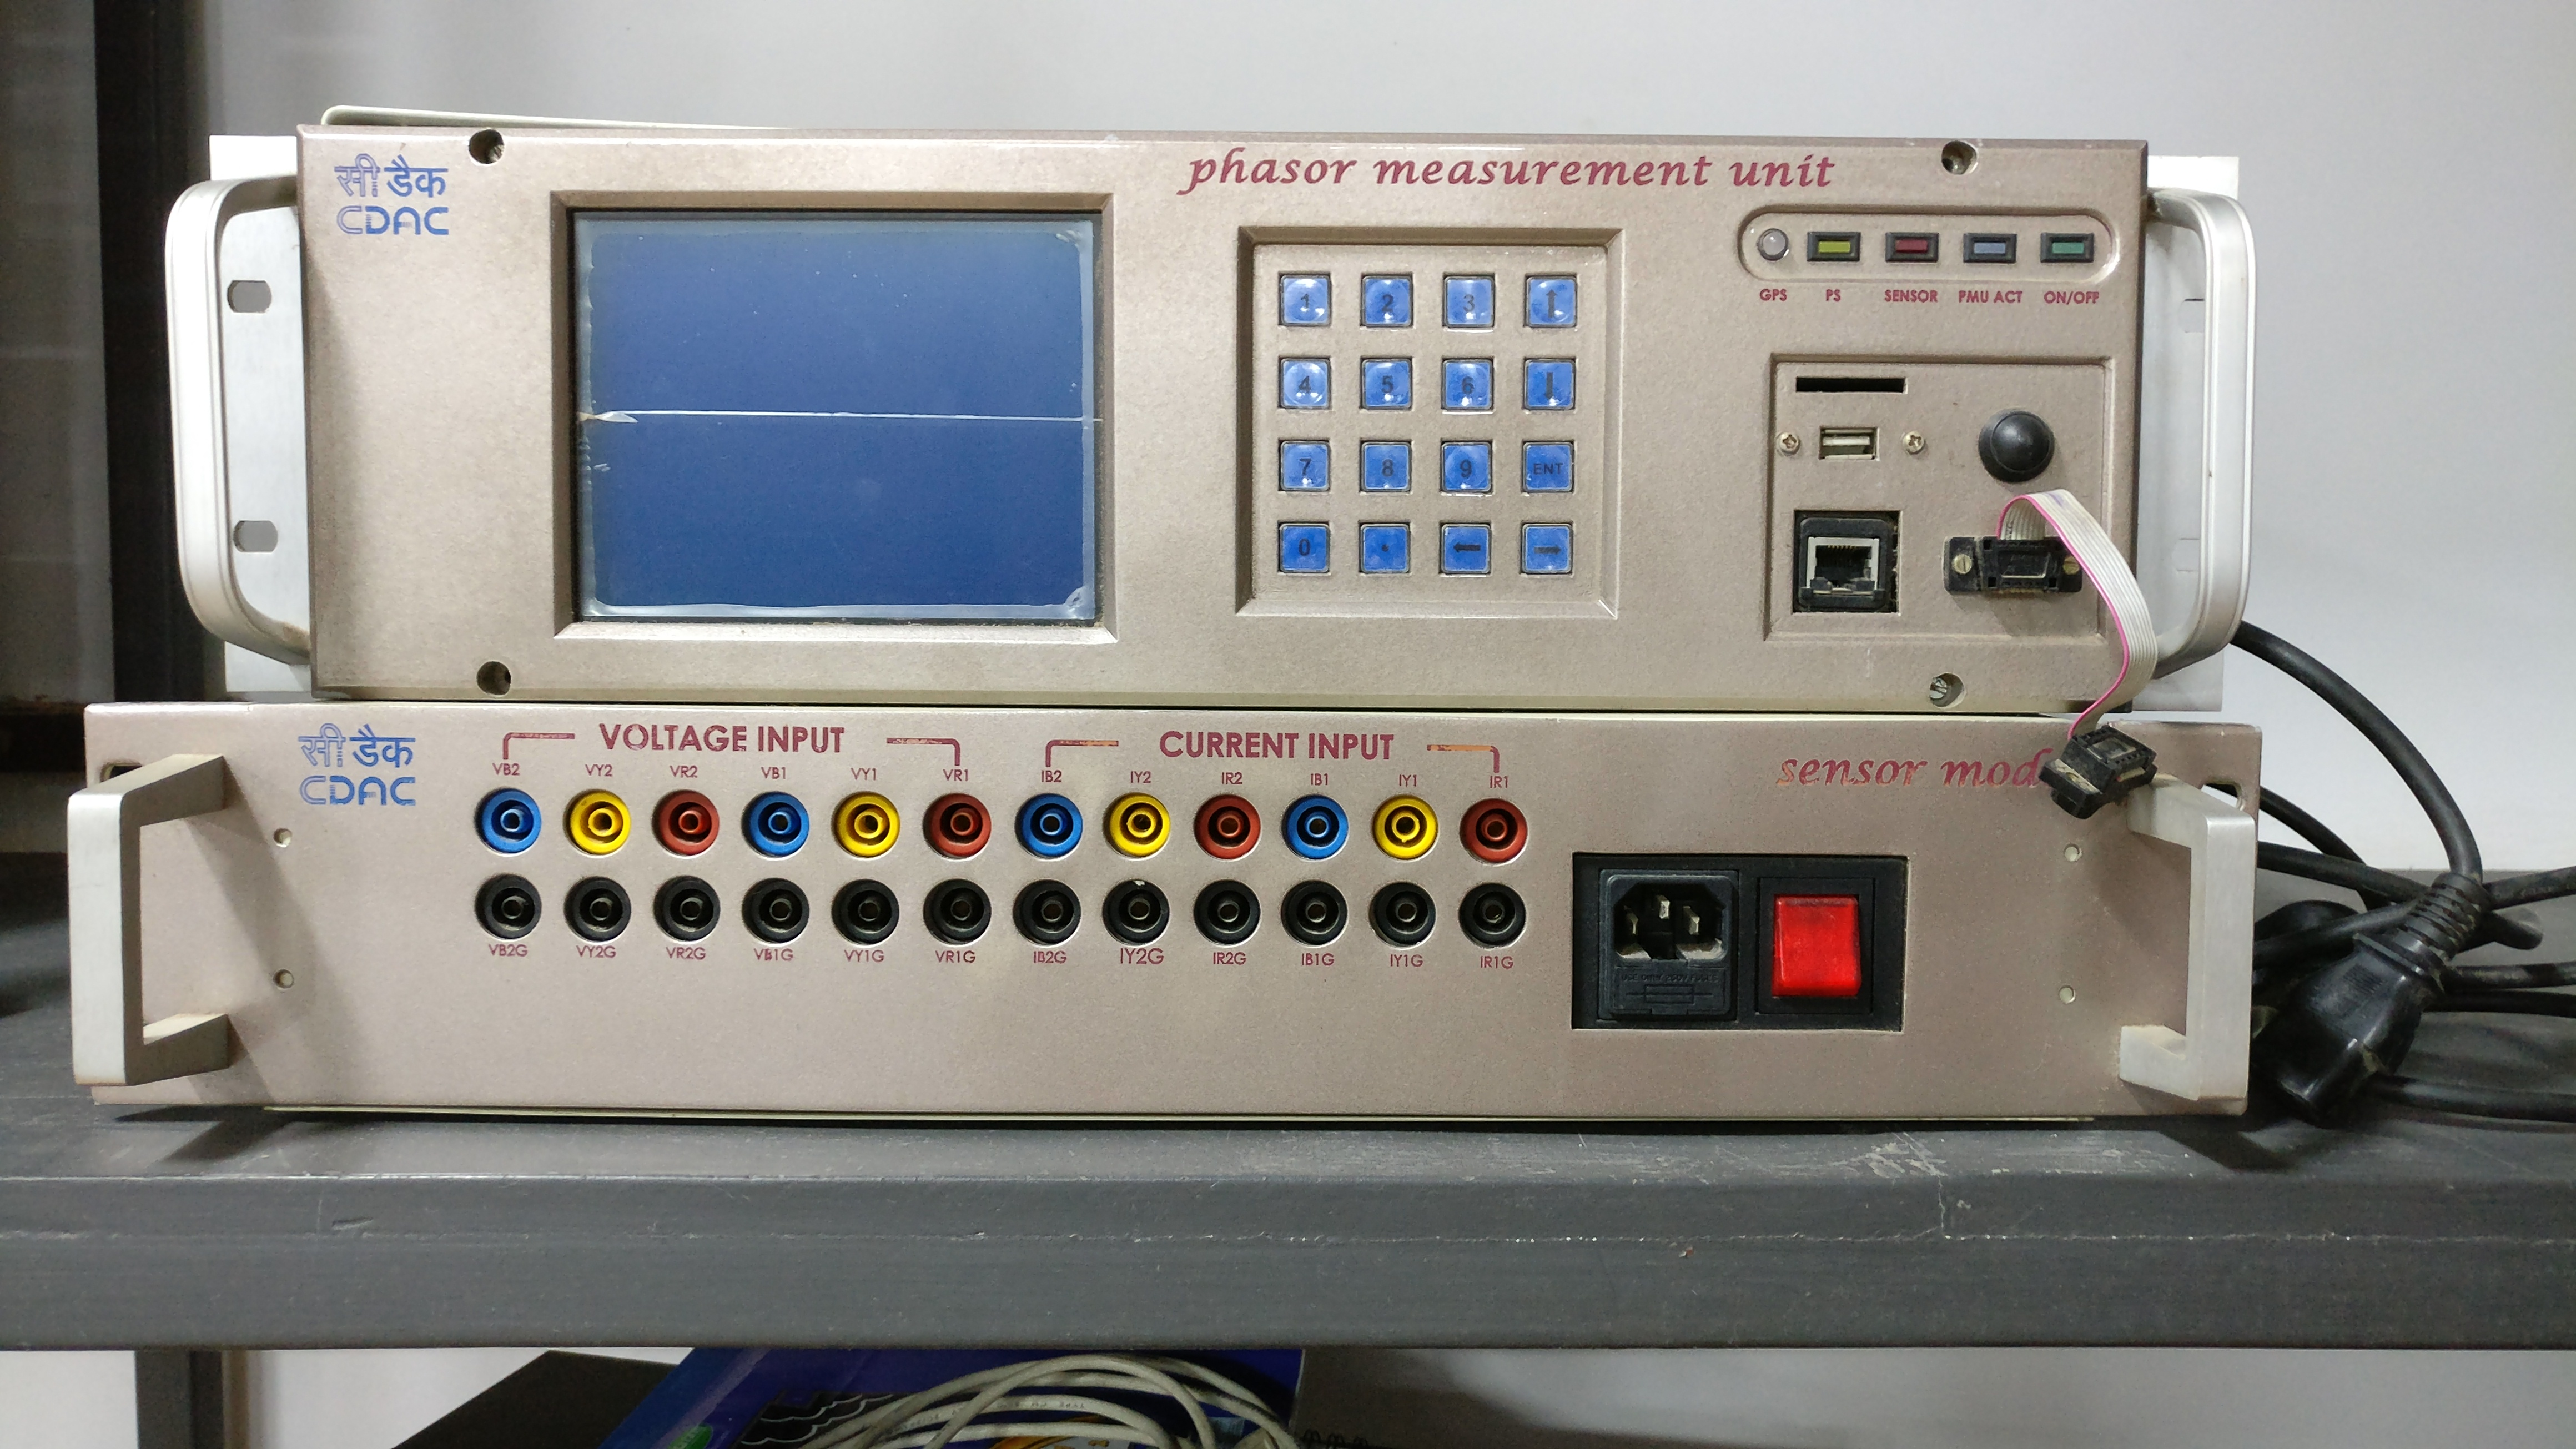
\includegraphics[width=\textwidth]{fig/cdac_pmu.jpg}
\caption{C-DAC, trivendrum PMU}
\label{fig:cdac_pmu}
\end{figure*}
